\newpage

\section{Model set-up and theories}

Apart from the free shear flows, most turbulent flows are bounded by one or more solid surfaces depending on whether they belong to class of the internal or external flow of fluids i.e. flow through pipes and flow over a car respectively.  In this investigation one of the simplest internal flow has been chosen for the validation \& testing of the implementation: fully developed channel flow. In this flow the mean velocity vector will be parallel to the wall and this flow is considered to be of prime importance as it has played a prominent role in the development of the study of the wall bounded turbulent flows~\cite{pope:book}.~\cite{pope:book} has described the fundamental theories of the full developed channel flow in great detail along with the reasoning of certain behaviour of the fluid near the channel wall.~\cite{froehlich:book} also has a good compilation on the fully developed channel flow. In general it serves as a very good reference for the beginners in LES.

In this section an attempt will be made to address the main challenges faced in the LES simulations that will include the mesh statistics, initialization, experimental settings, boundary conditions, LB solver specifics followed by post-processing and the final discussions of the results. 

\subsection{Turbulent channel flow}

Fully developed turbulent channel flow is a classic benchmark case and has been studied extensively to investigate and understand the mechanics of wall-bounded turbulent flows. It is the geometrical simplicity of this case that has lured to a large number of, computational (DNS) and experimental, investigations being carried out for the turbulent channel flow over the years and as a result, an adequate database (DNS data) for certain Re-numbers is already available.~\cite{channeldata:99}(MKM, Moin \& Jiminez) Link too. Historical progression in the turbulent channel flow simulations have been very well documented in the literature by Kim et al. Also, Kim has pointed out several difficulties related to the experimental measurements and how numerical simulations serve as an essential tool, alongside the experimental results, for the study of the wall-bounded turbulence. The recent development along with the comparison of the DNS results of the turbulent channel flow simulations for higher Re-numbers is documented in [Moser]
As shown in the figure a three dimensional flow through a rectangular duct is considered and the aspect ratio of the duct is $\gg$ than 1.
The dimensions of the 3d box are shown in the table~\ref{Computational Domain}

\begin{table}[!h]
\centering
\begin{tabular}{c|c}
\hline
$Nominal \ret$ & $L_x$ x $L_y $x $L_z$ \\
\hline
%
395   &  $6\de$ x $2\de$ x $3\de$  \\
\hline
\end{tabular}
\caption{The size of the domain in x, y, z directions}
\label{Computational Domain}
\end{table}

The size of the 3D duct has been chosen in accordance with the reference literature of ~\cite{moser:kim:mansour:99}.

\subsubsection{Governing equations}

Turbulent channel flow is fully developed, where the velocity statistics along the stream-wise direction remain constant i.e. ${\D U}/{\D x}=0 $, and statistically one dimensional, where the flow statistics vary only in the wall-normal(y) direction. Since the flow is two-dimensional, there is no mean flow in the span-wise direction i.e $W=0$ and thus the gradient of the span-wise velocity in the span-wise direction is zero i.e. ${\D W}/{\D z}=0 $. The mean continuity equation for the incompressible flow results in the mean wall normal velocity gradient to be zero:
\begin{equation}
\label{zero wall-normal mean vel. gradient}
\begin{split}
{\D V}/{\D y}&=0
\end{split}
\end{equation}
The eq.~\ref{zero wall-normal mean vel. gradient} when integrated, within the wall limits [0,$2\delta$], gives $V=const(y)$ and using the no-slip boundary condition, $U_i = 0$, applied at the walls results in $V = 0$. Now to satisfy the resulting continuity equation eq.~\ref{zero wall-normal mean vel. gradient}, $V$ has to be zero everywhere in the domain. Using the above made considerations and applying it to the mean stream-wise momentum equation we will have the following force balance:
\begin{equation}
\label{Forces channel flow}
\frac{\D \tau}{\D y} = \frac{\D P}{\D x}\\
\end{equation}
where $\tau = \left(\mu \frac{\D U}{\D y} - \rho\uij\right)$ is the total shear stress.\\

The eq.~\ref{Forces channel flow} shows that the total shear stress gradient and the pressure gradient balance each other in the full developed channel flow. It shows an equality of the form $\emph{f(x)}= \emph{g(y)}$ and for this equality to hold it is important that both $\emph{f(x)}$ and $\emph{g(y)}$ are individually constants. In eq.~\ref{Forces channel flow} both the gradients are dependent on different variables and thus they must be individually constants for this equality to hold. $$\frac{\D P}{\D x} = const\  \&\  \frac{\D \tau}{\D y} = const$$\\
%
Total shear stress is the summation of the viscous stress, $ \mu \frac{\D U}{\D y} $, and the Reynolds stress, $- \rho\uij$. At the wall with the no-slip boundary condition applied, the Reynolds stresses are reduced to zero and thus the shear stress near the wall or to be specific at the wall would entirely be dominated by the viscous stresses. Shear stress can be defined here as the \emph{wall shear stress},\marginpar{\bf wall shear \\stress} the region where the viscous stresses are dominant:
\begin{equation}
\label{Wall shear stress}
\begin{split}
\tau_w = \mu \frac{\D U}{\D y}\\
\tau\left(0\right) = \tau_w  = -\tau\left(2\delta\right)\\
\end{split}
\end{equation}\\
%
Now we can integrate the eq.~\ref{Forces channel flow}, from 0 to $2\delta$, for the pressure gradient and express the solution in terms of the $\tau_w$:
%
\begin{equation}
\label{Solution equations}
\begin{split}
-\frac{\D P}{\D x} = \frac{\tau_w}{\delta} \ ,\\
\end{split}
\end{equation}\\ 
%
From the fully developed channel flow it is known that the mean velocity profile (time-averaged) remains constant. It is clear from eq.~\ref{Wall shear stress} that wall shear stress is linearly proportional to the velocity gradient near the wall. A constant velocity profile implies that the wall shear stress will also be constant in a fully developed channel flow. Thus from eq.\ref{Solution equations} we can say that the pressure gradients is constant. $\tau\left(y\right)$ is anti-symmetric about the mid channel height $\tau\left(\delta\right)$ and thus the total shear stress is zero there. 
Integrating the eq.~\ref{Forces channel flow}, from 0 to some y, with the no-slip boundary condition at the wall results in the following solution:
\begin{equation}
\label{Shear stress profile}
\begin{split}
\tau\left(y\right) = \tau_w \left(1 - \frac{y}{\delta}\right)\\
\end{split}
\end{equation}\\ 
%
The pressure gradient in eq.~\ref{Solution equations} is negative as the viscous effects decreases the pressure along the stream-wise direction. It is this pressure gradient that drives the flow through the infinite parallel plates. For a given pressure gradient and the half-channel height we get a linear shear stress profile from eq.~\ref{Solution equations} and ~\ref{Shear stress profile} independent of the fluid properties and the state of the fluid motion (laminar or turbulent)~\cite{pope:book}.
Also, several investigations have showed that the total shear stress
profile is anti-symmetric about the channel mid height $ y=\delta $ and thus $\tau\left(\delta\right) = 0$.
%
\subsubsection{Scaling units}
The Reynolds stresses decreases towards the wall, remain zero at the wall and so does the eddy viscosity (\emph{Boussinesq hypothesis}). The value of the eddy viscosity ranges from zero, at the wall, to several orders of magnitude higher than the molecular viscosity, in the core region of the turbulent boundary layer~\cite{cengel:book}. From the figure. \ref{TFlow} it can be seen that the velocity profile changes more slowly (more flatter compared to the parabolic flow profile) in the core of the turbulent boundary layer, where the eddy viscosity is higher than the molecular viscosity, and there is an abrupt change in the velocity profile near the wall, where the molecular viscosity is dominant. The turbulent flow profile has the largest gradient near the wall. 
\begin{figure}[h]
    \centering
    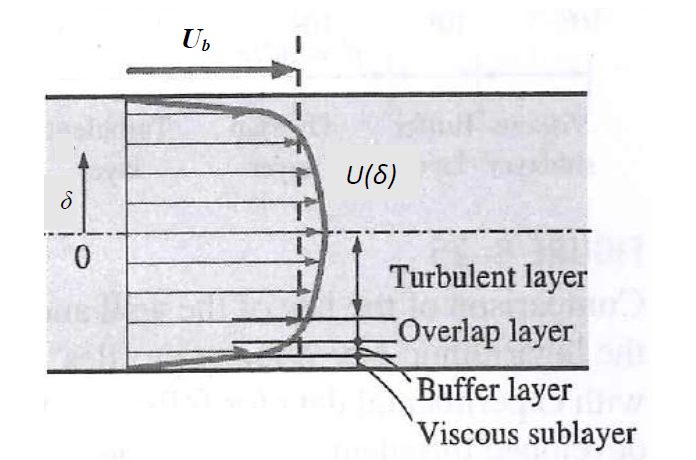
\includegraphics[width=0.6\textwidth]{figur/Turbulent_profile.png}
    \caption{Velocity profile in the fully developed channel flow ~\cite{cengel:book}}
    \label{TFlow}
\end{figure}

Turbulent flow along the wall can be considered to consist of four different layers, characterised by their distance from the wall. All four layers have been approximately shown in figure \ref{TFlow}. The layer closet to the wall is the viscous sub-layer, where the viscous effects are dominant. The velocity profile changes linearly with the distance from the wall and the flow is streamlined. Next to the viscous sub-layer is the buffer layer, where the turbulent stresses start to develop, but still the viscous stresses are dominant. Above the buffer layer is the overlap layer, where the turbulent stresses are significant, but still not dominant enough as the viscous stresses. The layer above the overlap layer for the rest of the flow is the outer or turbulent layer, where the turbulence stresses dominate over the viscous stresses.\\
%
A single analytical relation for the entire turbulent velocity profile is not suitable, as different regions or layers execute different flow characteristics. The best possible option is to find the key parameters or the functional forms using the dimensional analysis and later on experimental data can be used to obtain the numerical values of the any constants.\\

\textbf{i. Viscous sub-layer :} With the no-slip boundary condition applied at the wall, \emph{$u_i(0,t) = 0$}, the entire contribution to the shear stress is purely via viscous stresses i.e. $\tau_w$. From eq. \ref{Wall shear stress} it is clear that shear stress is proportional to the molecular viscosity. The thickness of this layer is very small, but it plays an important role on the flow characteristic because of the presence of large velocity gradients in it. The velocity profile remains linear in this layer and also it has been shown in certain experiments ~\cite{cengel:book}. Since the velocity profile is linear the gradient in the equation \ref{Wall shear stress} remains constant i.e. ${\D U}/{\D y} = {U}/{y} $. Thus the wall shear stress can be written as:
\begin{equation}
	\label{viscous sub-layer equ}
	\frac{\tau_w}{\rho} = \frac{\nu U}{y}
\end{equation}\\
Near the wall the important parameters are : $\tau_w$, $\rho$, $\nu$. The square root of the term on the left hand side has the dimensions of velocity and thus we define a new parameter as the \emph{\textbf{friction velocity}, $u_\tau$}:
\begin{equation}
	\label{friction velociy}
	u_\tau = \sqrt{\frac{\tau_w}{\rho}}
\end{equation}\\
Replacing $u_\tau$ in the eq. \ref{viscous sub-layer equ} we have \emph{\textbf{the law of wall}}:
\begin{equation}
	\label{law of wall}
	\frac{U}{u_\tau} =  \frac{u_\tau y}{\nu}
\end{equation}\\
The quantity $\nu / u_\tau $ has the dimensions of length and it is called \emph{\textbf{viscous length}} , $\delta_\nu$,  and it is used to nondimensionalze the distance from the wall, y. In the analysis of the boundary layer flow, it is convenient to work with the nondimensionalised distance and the velocity. The nondimensionalised quantities are represented with a $+$. \\
\emph{\textbf{Nondimensionalised variables} : } \begin{equation}
	\label{nondimensions}
	y^+ = \frac{y u_\tau }{\nu} \    and \    u^+ = \frac{U}{u_\tau}
\end{equation}\\
\emph{\textbf{Normalised law of the wall : }}\begin{equation}
	\label{nondimensions law of wall}
	u^+ = y^+ 
\end{equation}
This law shows a very good correlation with the experimental data for smooth surfaces for $0\leq {u_\tau y}/{\rho} \leq 5	$. Thus for the $y^+ =  5$ we will have the linear velocity profile and the viscous sub-layer. \\

\begin{figure}[t]
    \centering
    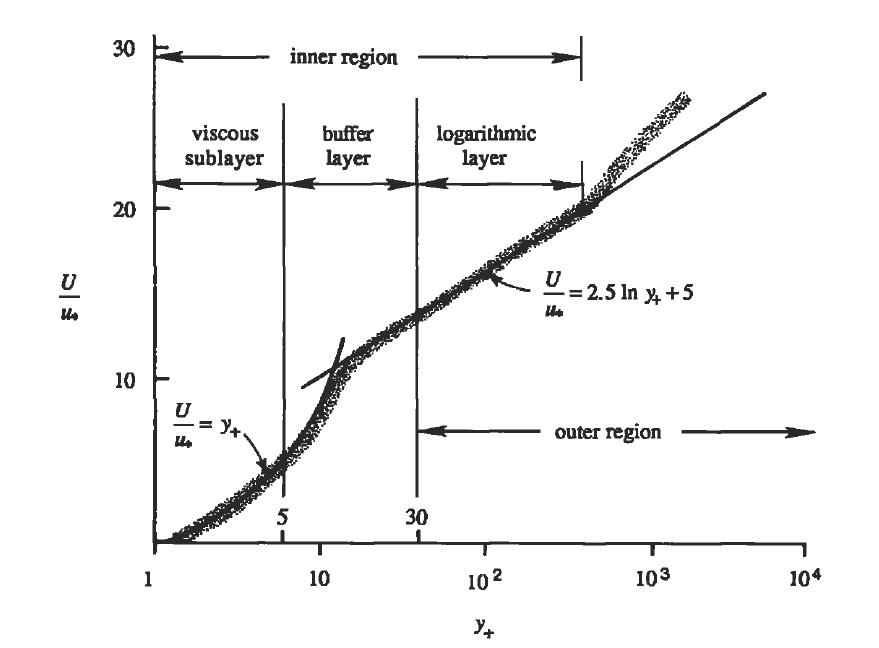
\includegraphics[width=0.9\textwidth]{figur/Log-law-plot.png}
    \caption{Nondimensional velocity $u^+$ vs. the nondimensional distance $y^+$ (plotted in logarithmic scale) ~\cite{kundu:book}}
    \label{log-log plot}
\end{figure}


\textbf{ii. Overlap layer:} From the dimensional analysis and the experimental results it proved that the velocity in the overlap region is proportional to the logarithm of distance and it can be expressed as: 
\begin{equation}
	\label{log law}
	u^+ = \frac{1}{\kappa}\ ln\ y^+ + \ B \ or \  u^+ = 2.5\ ln\ y^+ + \ 5.0 
\end{equation}
where $\kappa$ and $B$ are constants and equal to 0.40 and 5.0 respectively. The eq. \ref{log law} is called the \emph{logarithmic law} and the overlap layer is also called as the \emph{logarithmic layer} or \emph{log-law layer}. It is clear from the figure \ref{log-log plot} that the eq. \ref{log law} represents the experimental data quite satisfactorily from $y^+ \geq 30$ till outer region. Neither eq. \ref{log law} nor the eq. \ref{law of wall} represents the experimental data satisfactorily in the buffer layer.
From Figure. \ref{log-log plot} it is seen that :\\

\emph{\textbf{viscous sub-layer}	} : $y^+ \leq  5$ \\ 

\emph{\textbf{buffer layer}} : $y^+ \geq  5$ till $y^+ \leq  30$ \\

\emph{\textbf{logarithmic layer}} : $y^+ \geq  30$ till $y^+ \leq  10^3$ \\\\
%
\textbf{iii. Outer layer:} The velocity law for this region is:
\begin{equation}
	\label{vel defect law}
	\frac{\left(U_{max} - U\right)}{u_\tau} = \frac{1}{\kappa}\ ln\ \left(\frac{y}{\delta}\right)  
\end{equation}
The difference between the mean center line velocity, $U_{max}$, and the mean velocity, $U$ is called the \emph{\textbf{velocity defect}} and thus this law is called the \emph{\textbf{velocity defect-law}}. In this region the turbulent stresses are dominant compared to the viscous stresses and this is also seen from the eq. \ref{vel defect law}: the normalised velocity profile in the core region of the turbulent channel flow is dependent on the half-channel height and is not dependent on the viscosity. 

\subsection{Reynolds number}
Since the Reynolds number is used to characterize the flow, great care was taken to simulate the same flows i.e. same Reynolds number as that of the DNS data was used. The dimensionless Reynolds number requires three parameters for its definition: characteristics length ($\delta$), characteristic velocity ($V_{ch}$) and the kinematic viscosity ($\nu$) of the fluid. 
$$ Re = \frac{V_{ch}\delta}{\nu} $$
Several choices of $V_{ch}$ are possible, but in this investigation two different $V_{ch}$ have been chosen and the respective Reynolds number are as follows :\\

\textbf{i. Friction Reynolds number ($Re_\tau$):}\begin{equation}
	\label{friction Re}
	Re_\tau = \frac{u_\tau \delta}{\nu}  = \frac{\delta}{\delta_\nu}  
\end{equation}

\textbf{ii. Bulk Reynolds number ($Re_b$):}\begin{equation}
	\label{bulk Re}
	Re_b = \frac{U_b\ 2\delta}{\nu}
\end{equation}
The bulk mean velocity is defined as:
$$U_b = \frac{1}{h}\int_{0}^h U dy$$

\subsection{Computational Domain and Meshing}
\subsubsection{Computational Domain}
We are interested to investigate the fully developed turbulent channel and that implies a sufficient length and width of the domain for the flow in the channel to be fully developed. Since the stream-wise and the span-wise directions are homogeneous, periodic boundary conditions are applied on either side of the two homogeneous directions. All flow properties along with the state of the flow are set to be equal for the equivalent points on the periodic boundary pairs. Use of periodic boundaries is equivalent to having an infinitely long domain in that direction. This implies that we have a flow between two infinite parallel planes, Figure \ref{infinite plates}.
%
\begin{figure}[h]
    \centering
    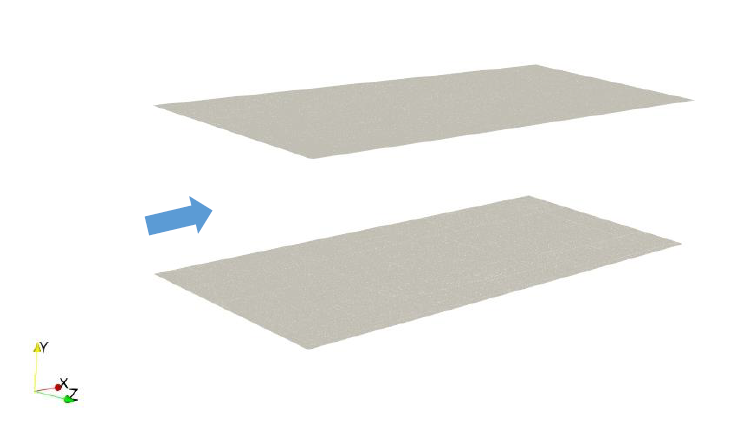
\includegraphics[width=0.9\textwidth]{figur/Infinite_plates.png}
    \caption{Flow between the infinite parallel plates}
    \label{infinite plates}
\end{figure}
%
Since the artificial periodic boundaries are enforced great care has to be taken that the domain is long enough to avoid this artificial boundary conditions from influencing the results.\emph{Moin et.al}~\cite{Moin:78} has specified certain aspects to be considered in the process of choosing the dimensions of the flow domain for the numerical simulation of the turbulent channel flow. According to~\cite{Moin:78} the experimental two-point correlation functions have to be considered for choosing the stream-wise $\left(L_x\right)$ and the span-wise $\left(L_z\right)$ lengths. The usage of periodic boundary conditions is justified if the distance between the pair of periodic boundaries is at least twice the distance, at which the correlation function becomes zero. This means that the domain size is enough to accommodate the largest eddy without the pair of periodic boundaries influencing each other.\\

To validate the LES results of the fully developed turbulent channel flow the DNS data from the database of~\cite{moser:kim:mansour:99} for the $Re_\tau = 395$ is used. The authors have shown the adequacy of the domain by performing the two-point spatial correlations. Same domain size used in~\cite{moser:kim:mansour:99} has been chosen for performing the LES of channel flow, Table \ref{Computational Domain}. Thus, no separate study for two-point correlation has been performed in this investigation.
%
\begin{table}[!h]
\centering
\begin{tabular}{c|c}
\hline
$Nominal \ret$ & $L_x$ x $L_y $x $L_z$ \\
\hline
%
395   &  $2\pi\de$ x $2\de$ x $\pi\de$  \\
\hline
\end{tabular}
\caption{The size of the domain in x, y, z directions}
\label{Computational Domain}
\end{table}\\
%
Several authors ~\cite{Freitas:11, sonja:12} have performed the turbulent channel flow simulations with smaller domain dimensions comapred to the dimensions used in the reference data, ~\cite{moser:kim:mansour:99}, in order to save the computational time. But \emph{Bespalko}~\cite{bespalko:11} suggests that for performing the validation studies the dimensions of the domain should be similar to that used in the reference data. Else, the usage of smaller domain dimensions might add some kind of error and this might be than attributed to the error originating from the implementation under test.

\subsubsection{Physical parameters}
The physical parameters that are necessary for the model set-up and later on for the simulations are pressure gradient(to drive the flow), discussed in the later section, $u_\tau$, $\nu$ and $U_b$
In ~\cite{moser:kim:mansour:99} the authors have not specified $u_\tau$, $\nu$ and $U_b$ used in the simulations.~\cite{devilliers:phd} has computed and specified these parameters obtained from the DNS results of ~\cite{moser:kim:mansour:99} for $Re_\tau = 395$, Table \ref{Physical quantities}  :

%
\begin{table}[!h]
\centering
\begin{tabular}{c|c|c}
%\hline
$ $ & $Value\ in\ S.I\ Units$ & $Expression$ \\
\hline
%
Half channel height, $\de$ & $1.0\ m$ & $9437184$ \\
\hline
%
Friction velocity, $u_\tau$ & $0.0079\ m/s$ & $ $ \\
\hline
%
Bulk velocity, $U_b$ & $0.1335\ m/s$ & $ $ \\
\hline
%
Kinematic Viscosity, $\nu$ & $0.00002\ m^2/s$ & $ $ \\
\hline
%
\end{tabular}
\caption{Physical quantities}
\label{Physical quantities}
\end{table}
%
 
In order to compute the bulk mean velocity from the DNS data (Mean stream-wise velocity), trapezoidal rule can be used to solve the equation of $U_b$ numerically. i.e. \emph{trapz} command in Matlab. 
\subsubsection{Meshing}
In order to see the effects of mesh resolution a hierarchy of meshes was created. Three uniformly spaced meshes, in all directions, were generated namely: Mesh 1 (coarse), Mesh 1\_5 (medium) and Mesh 2 (fine). The resolution of Mesh 1 was refined by a factor of 1.5 in all directions for Mesh 1\_5 and similarly by a factor of 2 for Mesh 2. To compute the mesh spacing the dimensionless distances in wall normal and wall parallel directions (stream-wise and span-wise) were used. Initially the plan was to go for Mesh 3, refinement by factor 4 in all directions, but the total number of mesh points were $\sim 88\ million$ ,so the idea was dropped and an intermediate mesh resolution was chosen and hence the name Mesh 1\_5.
\begin{equation}
\label{Dimensionless distances}
\begin{split}
x^+ = \frac{\Delta x u\tau}{\nu}\\
y^+ = \frac{\Delta y u\tau}{\nu}\\
z^+ = \frac{\Delta z u\tau}{\nu}\\
\end{split}
\end{equation} 
Since the spacing is same in all three directions from now onward it will be referred as $\Delta^+$. The bottom and top faces of the domain were defined as the wall, no-slip boundary condition. The no-slip boundary condition was realized by using the half-way bounce back boundary condition. Because of the half-way bounce back boundary condition the distance of the nearest cell to the wall, $y^+$, is halved. The $y^+$ will always be a smaller than $\Delta^+$ by a factor of 2. The following table \ref{Mesh statistics} shows the mesh statistics used in the investigation, where $N_x\ , N_y\ , N_z$ denote the number of nodes in the stream-wise, wall-normal and span-wise directions. In order to facilitate the grid generator the size of domain was reduced to $6\de$ x $2\de$ x $3\de$.
%
\begin{table}[!h]
\centering
\begin{tabular}{c|c|c|c|c}
%\hline
$ $ & $N_x$ x $N_y$ x $N_z$ & $Total\ nodes$ & $\sim \Delta^+$ & $\sim y^+$ \\
\hline
%
Mesh 1 & $192$ x $64$ x $96$ & $1179648$ &$12$ & $6$ \\
\hline
%
Mesh 1\_5 & $288$ x $96$ x $144$ & $3981312$ & $8$ & $4$   \\
\hline
%
Mesh 2 & $384$ x $128$ x $192$ & $9437184$ &$6$ & $3$ \\
\hline
%
\end{tabular}
\caption{Mesh statistics}
\label{Mesh statistics}
\end{table}\\
%
The domain size has been slightly altered in this investigation and this leads to the necessity for performing the two-point correlations to prove the adequacy of the domain. \emph{Premnath et.al}~\cite{Premnath:09} suggests doing it otherwise.
%
%%%%%%%%%%%%%%%%%%%%%%%%%%%%%%%%%%%%%%%%%
%
\subsection{Initial conditions}
It is known from the theory of the internal fluid flow that there exists a hydrodynamic entry length ($L_h$), starting from the inlet (x = 0), that the fluid has to travel, in the channel, for the flow to become fully developed. This means when we integrate the flow governing equations, in time, the fluid has to travel the distance $L_h$ ($\tilde{x} =10H$) in every time-step, to generate a fully developed flow, which is unnecessary considering the computational efforts and also the storage requirements. The idea is to consider only that portion of the channel which will be fully developed, turbulent and not the initial part ($L_h$) of the channel. This implies we will have to provide specific initial conditions for the flow to become fully developed and turbulent.\\
%
Different approaches have been used by different authors to generate the initial condition for the incompressible, three-dimensional, unsteady, turbulent channel flow simulations.\emph{Moin et.al}~\cite{Moin:78} has specified few consistency criteria for initial velocity field. \emph{Sagaut}~\cite{sagaut:02} \& \emph{Fröhlich}~\cite{froehlich:book} have a concide description of most commonly used approaches with their respective advantage, disadvantages and their applications to suitable flows. Few of the several approaches mentioned in~\cite{sagaut:02} \& ~\cite{froehlich:book} will be discussed here.

\textbf{i. First approach:} In this approach a simulation is performed for some Reynolds number smaller than the one to be simulated. The resulting fields of this simulations are then used as the starting point for the required Reynolds number and is  simulated further in time until a steady state, where the statistics of the flow do not change with time, is achieved. This approach is termed as \emph{Precursor simulation} in several literature.

\textbf{ii. Second approach: } In this approach a laminar flow is chosen as the base flow and certain set of disturbances are applied on the base flow. The base flow super-imposed with disturbances is then integrated in time until the flow transitions to a turbulent flow. This approach is computationally intensive, as the flow takes time to become turbulent. There are several options available to impose the disturbances on to the base flow. Several authors have used this approach for the generating appropriate initial conditions. In this investigation this approach has been used.\\

For the initialisation of our simulations the work of \emph{Eugene de Villiers}~\cite{devilliers:phd} is closely followed. \emph{Eugene de Villiers} introduced some sort of near wall streak cycle, where he uses the fundamentals of the turbulent structures near the walls. A parabolic flow profile is chosen as the base flow. To generate the parabolic flow profile the bulk mean velocity, $U_b = 0.1335\ m/s$, which was computed by \cite{devilliers:phd}, from the mean velocity DNS data of \cite{moser:kim:mansour:99} for $Re_\tau = 395$, is used.\\

Parabolic flow profile has been applied in the stream-wise direction, $u(y,0)$,  on all the fluid nodes in the domain. Figure \ref{para profile} shows the parabolic profile used as the base flow. A combination of sine and cosine waves have been used to break the flow symmetry and to develop the turbulence in the flow. 
%
\begin{figure}[h]
    \centering
    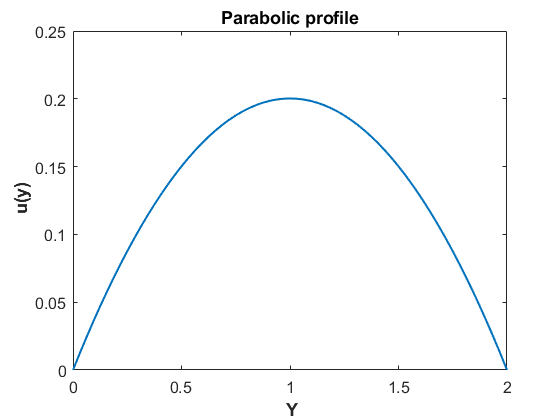
\includegraphics[width=0.6\textwidth]{figur/Parabolic_profile.png}
    \caption{Parabolic flow profile with $U_b = 0.1335\ m/s$}
    \label{para profile}
\end{figure}
Initially the the disturbances were applied the disturbance in the stream-wise direction, but that approach was quite time consuming. It took approximately 4.5 million time-steps for the flow to be turbulent. In the next approach we applied the disturbances in the wall-normal direction, $v$. This approach reduced the time it took for the flow to be turbulent, ~100,000 time-steps. The exact equations for the initialization have been specified in the the eq. \ref{Initial conditions} in Appendix.

\subsection{Solver settings}
In this subsection the modelling of the pressure gradient, which is the flow driving factor, along with the simulation settings for the LES will be discussed.

\subsubsection{Modelling of pressure gradient}


 
